\documentclass[10pt,a4paper]{extarticle}
\usepackage[margin=1.6cm,top=1.4cm,bottom=1.4cm]{geometry}
\usepackage{fontspec}
\setmainfont{Apple SD Gothic Neo}
\usepackage{graphicx,booktabs,xcolor,enumitem,titlesec,array}
\XeTeXlinebreaklocale "ko"
\XeTeXlinebreakskip=0pt plus 1pt
\setlength{\parindent}{0pt}\setlength{\parskip}{4pt}
\titleformat{\section}{\large\bfseries\color[HTML]{B3261E}}{}{0pt}{}
\titlespacing{\section}{0pt}{8pt}{3pt}
\setlist{nosep,leftmargin=1.3em}
\begin{document}
{\LARGE\bfseries 합정역 도로망: 시나리오가 일어나는 곳과 도로 구조}\hfill 2026-11-13

\vspace{3pt}\hrule\vspace{6pt}
\textbf{한 줄 요약.} 버스가 합정역에서 출발해 한 바퀴(약 1.9km) 도는 동안 여섯 가지 상황을 최대한 자주 만나도록 도로를 설계했다.
실제 지도에 있는 골목을 살려 버스 경로로 차가 나오는 곳을 여덟 곳으로 늘렸고, 골목에서 버스 앞으로 합류하는 차가 시간당 34대에서 218대가 됐다. 그런 다음 차가 다니지 않는 길을 지우고 신호를 고쳐, 드문 충돌과 정체를 300회 점검 기준 17회에서 7회로 줄였다. 마지막으로 길 전체를 다시 점검했고, 끊긴 길과 차가 다니지 않는 골목은 없다.

\section{1. 버스가 달리는 길}
버스는 합정역 사거리에서 출발해 독막로를 따라 상수역까지 간다. 상수역 사거리에서 좌회전해 와우산로로 올라가고, 삼거리포차 앞에서 다시 좌회전해 잔다리로를 지난다.
서교동사거리에서 세 번째 좌회전을 해 양화로로 합정역에 돌아온다. 이 경로 위에 실제 위치의 정류장 여섯 곳과 신호 없는 횡단보도 한 곳이 있다.

\begin{center}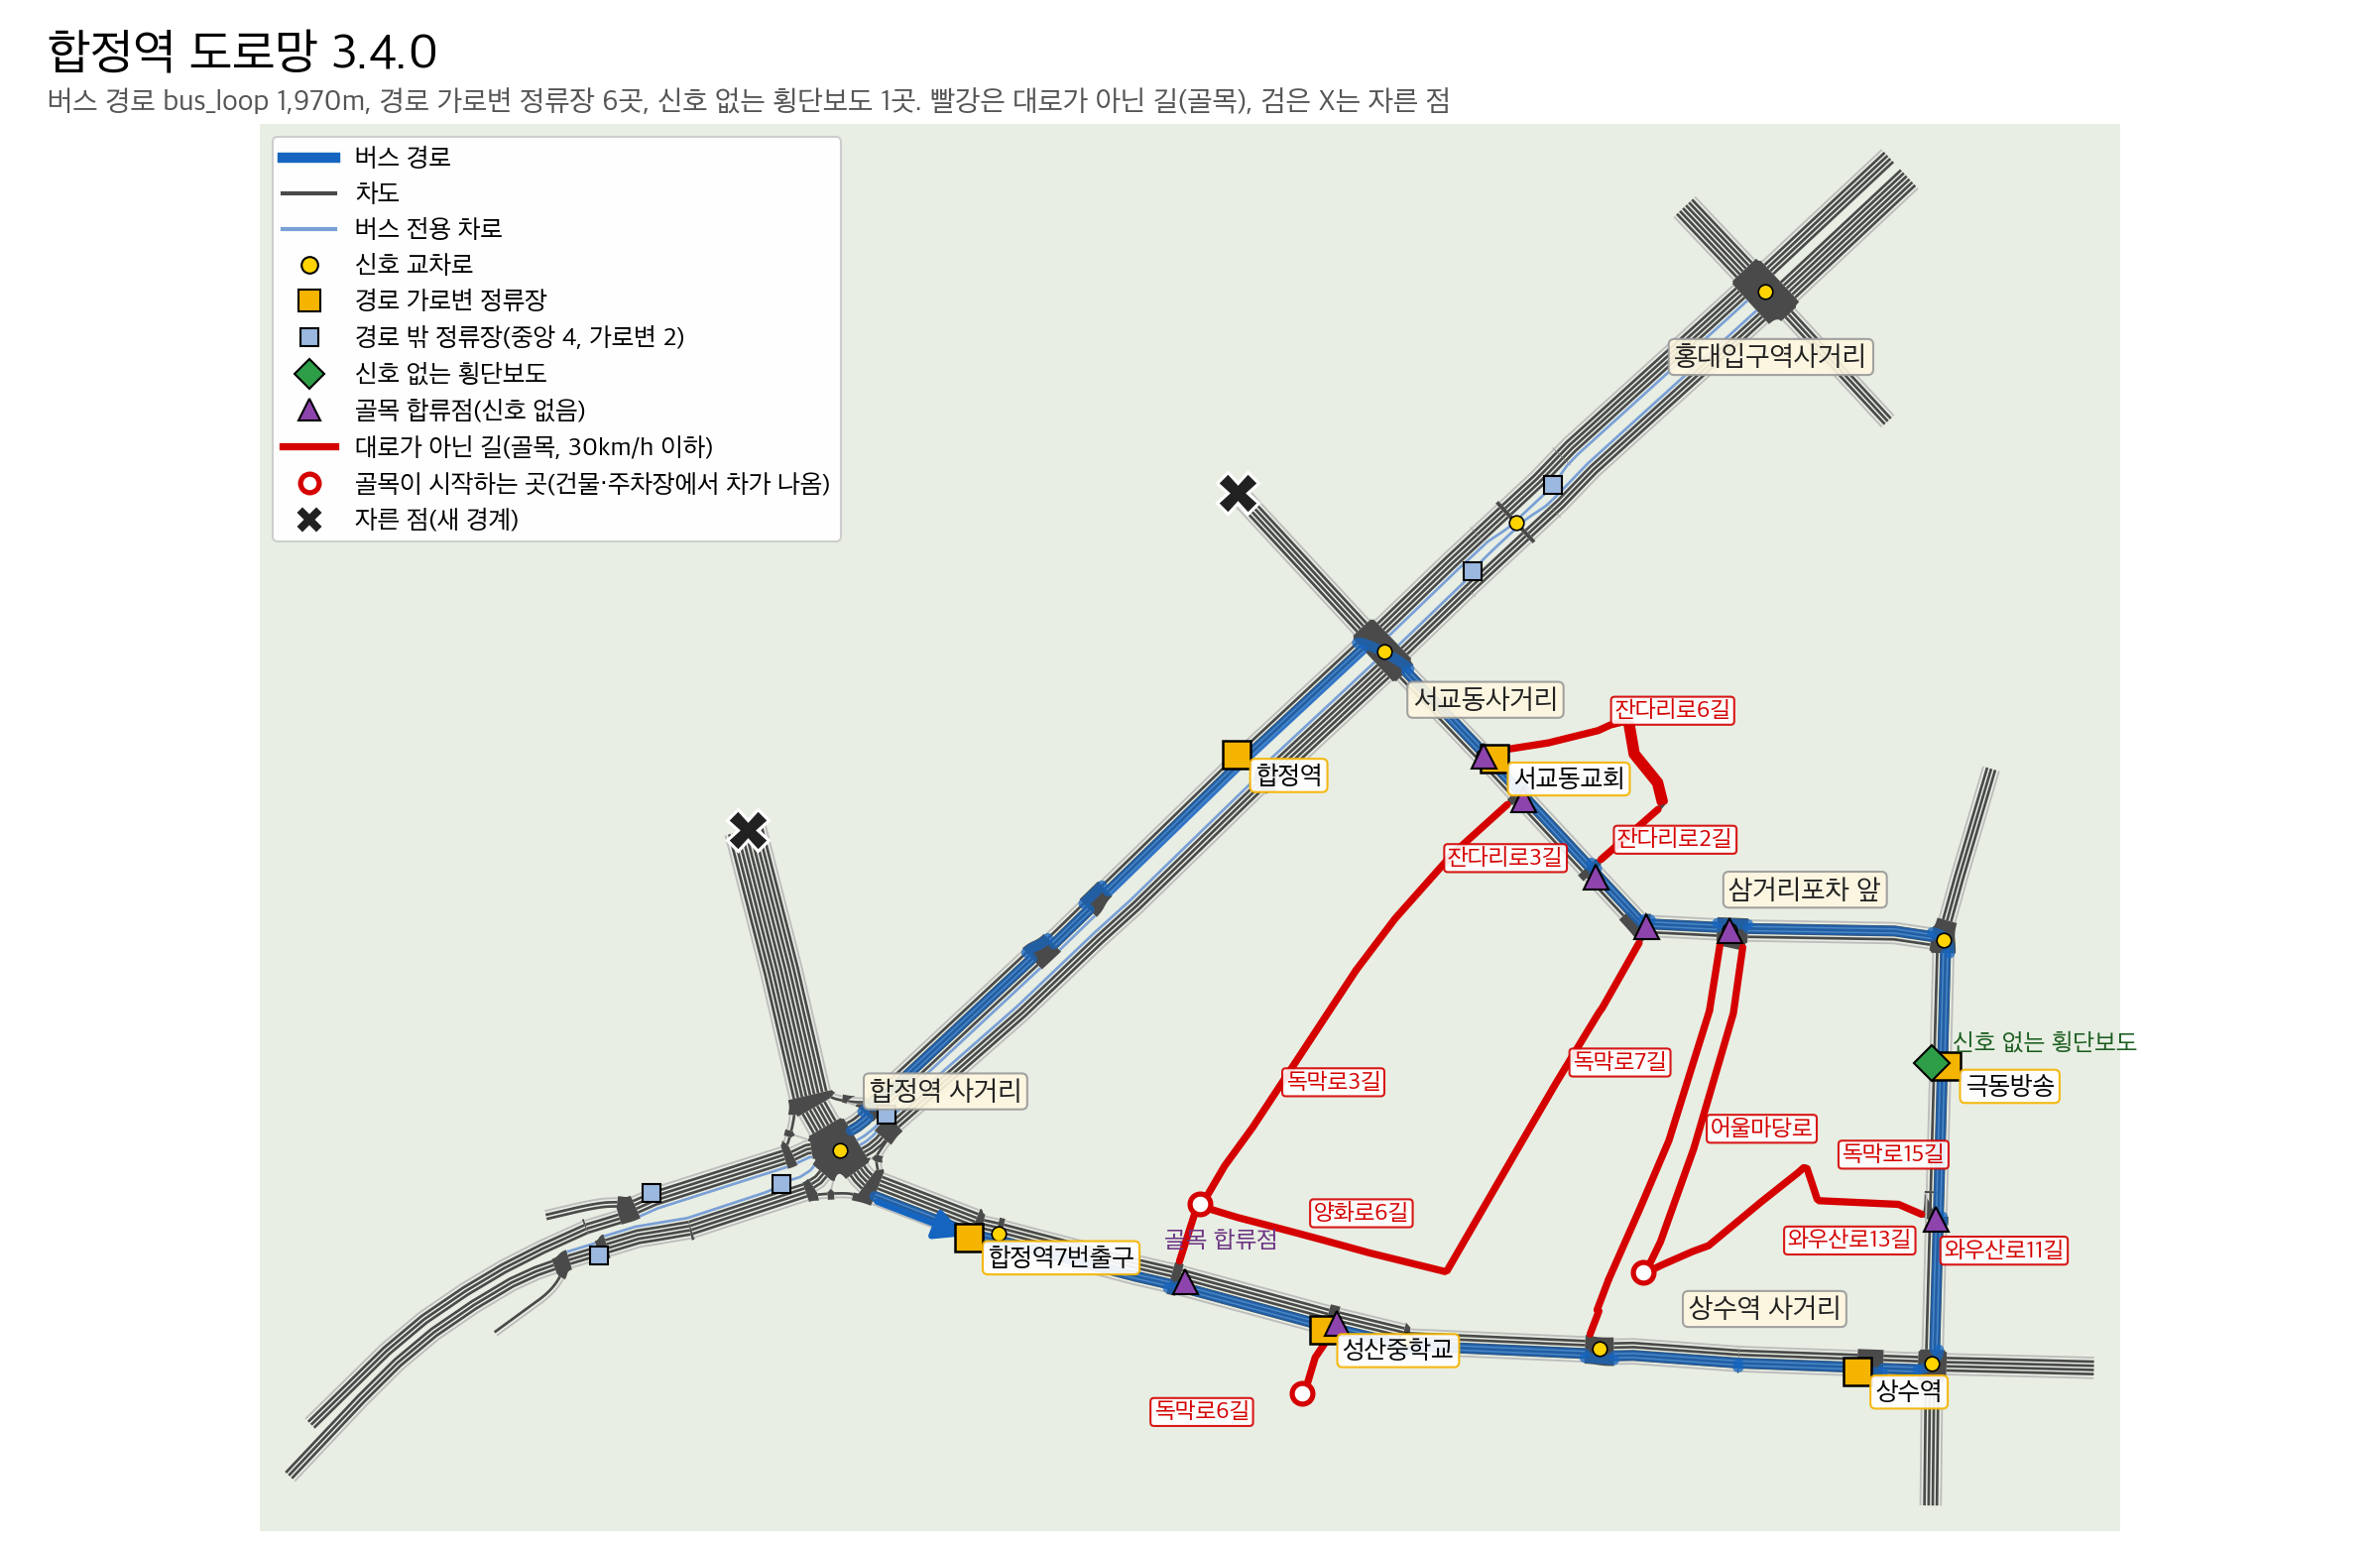
\includegraphics[width=0.97\textwidth]{road_map.png}\end{center}

\textbf{그림 읽는 법.} 파란 선이 버스 경로다. 노란 네모는 버스가 지나는 정류장, 노란 점은 신호 교차로, 초록 마름모는 신호 없는 횡단보도다.
빨간 선은 대로가 아닌 길(골목)이다. 빨간 테두리의 흰 동그라미는 골목이 시작하는 곳, 보라 세모는 골목이 버스 경로에 신호 없이 닿는 곳(합류점)이다. 검은 X는 도로망을 잘라낸 경계다.

\section{2. 도로는 네 겹으로 되어 있다}
\begin{tabular}{@{}>{\bfseries}p{2.9cm}p{14.3cm}@{}}
간선 도로 & 양화로, 독막로, 와우산로, 잔다리로. 버스가 달리는 길이고 교차로마다 신호가 있다. 제한속도는 시속 50km다. \\[2pt]
버스전용차로 & 양화로 가운데의 중앙버스전용차로. 실제 도로 규칙 그대로다. 일반 차는 들어가지 못한다. 연구 버스는 가로변 노선이라 이 차로를 쓰지 않는다. \\[2pt]
골목(빨간 선) & 독막로7길, 잔다리로3길, 어울마당로, 잔다리로6길·2길, 와우산로11길 등. 모두 실제 지도에 있는 길이고 신호가 없다. 제한속도는 시속 30km다. 모두 일방통행이고, 차가 실제로 다니는 방향만 남겼다. 골목이 시작하는 곳은 건물과 주차장에서 차가 나오는 곳이다. \\[2pt]
보행자 & 인도와 횡단보도. 교차로의 횡단보도는 신호를 따르고, 와우산로 중간의 횡단보도 한 곳은 신호가 없다. \\
\end{tabular}

\newpage
\section{3. 여섯 시나리오는 어디서 일어나는가}
\begin{center}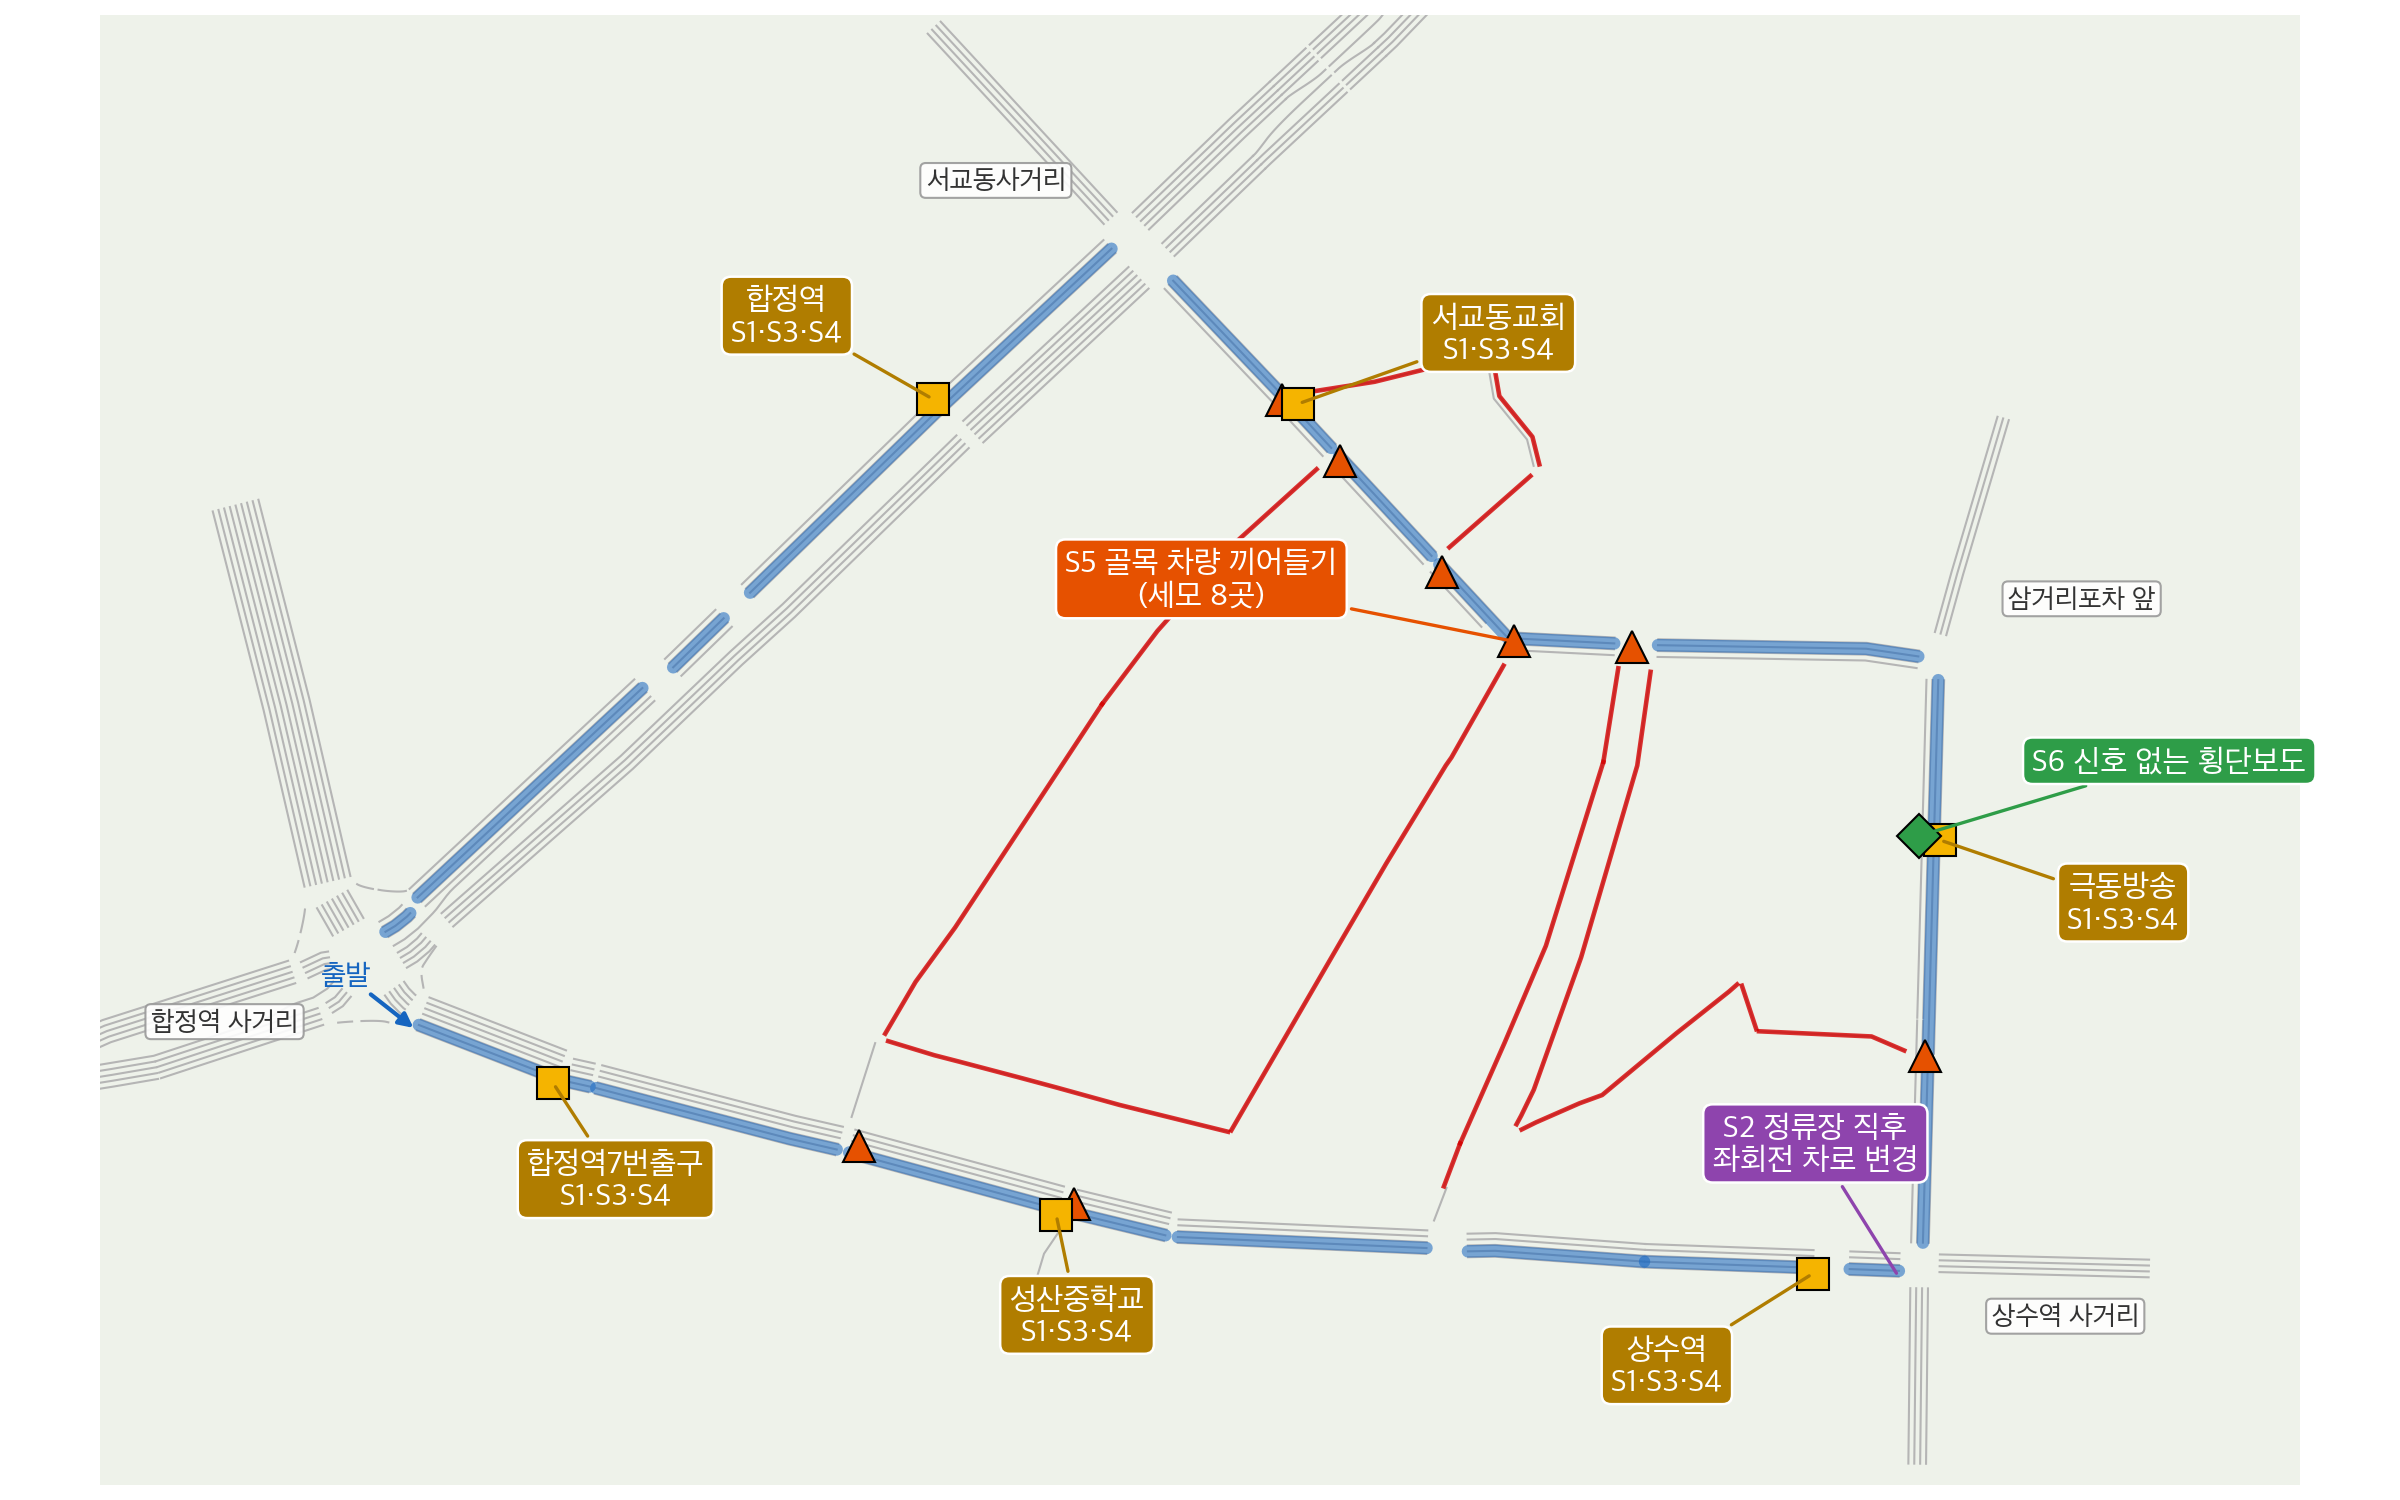
\includegraphics[width=0.99\textwidth]{scenario_map.png}\end{center}

\begin{tabular}{@{}>{\bfseries}p{4.3cm}p{6.6cm}p{6.0cm}@{}}
\toprule
시나리오 & 어디서, 왜 일어나는가 & 지금 얼마나 일어나는가 (버스 80회 주행) \\
\midrule
S1 정류장 출발 후 재합류 & 정류장 여섯 곳. 버스가 정류장에서 다시 차로로 나올 때 옆 차로의 차와 마주친다 & 정류장을 지날 때 옆에 차가 있던 경우 474번 중 210번. 버스가 아직 정류장에 서지는 않는다 \\[2pt]
S2 정류장 직후 좌회전 차로 변경 & 상수역 정류장 직후. 상수역 사거리에서 좌회전하려면 바로 왼쪽 차로로 옮겨야 한다 & 47회. 그중 옮겨 갈 차로에 차가 있던 것이 5회 \\[2pt]
S3 정류장 접근 차로 변경 & 정류장 여섯 곳의 앞. 바깥 차로로 옮겨 정류장에 붙는다 & S1과 같은 숫자(정류장 주변의 차)가 재료다 \\[2pt]
S4 정류장 앞 정차 차량 & 정류장 여섯 곳. 택시 같은 차가 정류장 앞에 잠시 선다 & 도로에는 자리만 있다. 정차 차량은 교통 담당 코드가 넣는다 \\[2pt]
S5 골목 차량 끼어들기 & 골목이 버스 경로에 닿는 여덟 곳. 골목 차가 신호 없이 버스 앞으로 나온다 & 골목에서 버스 방향으로 나오는 차 시간당 218대. 버스 앞 50m 안으로 끼어든 것 33번, 그중 버스와 같은 차로가 4번 \\[2pt]
S6 신호 없는 횡단보도 & 와우산로 극동방송 정류장 옆. 보행자가 신호 없이 건넌다 & 버스가 다가올 때 보행자가 건너려고 서 있던 것 72회, 건너는 중이던 것 1회 \\
\bottomrule
\end{tabular}

\vspace{4pt}
\textbf{구간마다 다른 상황이 나오게 했다.} 독막로에서는 정류장과 차로 변경(S1\textasciitilde S3)이, 와우산로에서는 횡단보도(S6)와 극동방송 앞 골목(S5)이, 잔다리로에서는 골목 다섯 곳의 끼어들기(S5)가,
서교동사거리 앞에서는 좌회전을 기다리는 줄로 끼어드는 차가 나온다. 한 바퀴를 돌면 여섯 가지를 고루 만난다.

\newpage
\section{4. 실험으로 고른 도로}
길 하나, 설정 하나를 넣을 때마다 같은 방법으로 재고 넣을지 정했다. 배경 차량만 한 시간씩 세 번 흘려 골목에서 나오는 차를 세고, 규칙대로 달리는 버스를 80번 돌려 버스가 실제로 겪은 일을 셌다.
마지막에는 30분짜리 점검을 300번 돌려 사건이 난 자리마다 원인을 찾아 고쳤다.

\begin{center}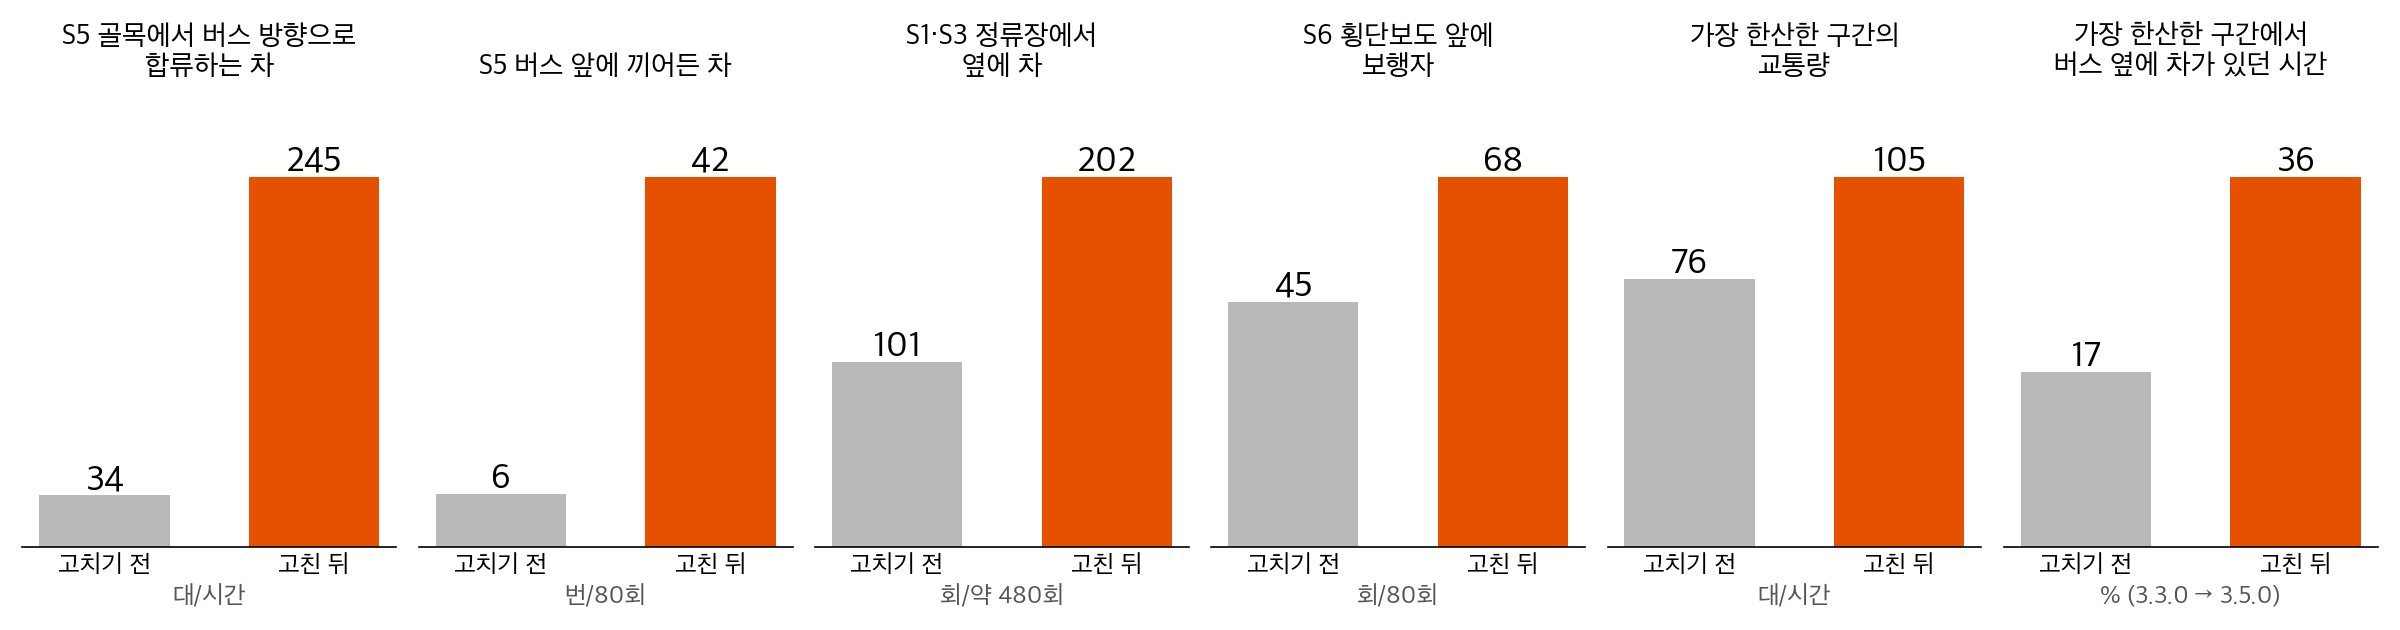
\includegraphics[width=0.9\textwidth]{progress.png}\end{center}

\textbf{넣은 것과 근거.}
\begin{itemize}
\item \textbf{골목 여섯 길.} 다 넣은 뒤 하나씩 빼 보니, 어느 길을 빼도 골목에서 나오는 차가 시간당 10\textasciitilde 23대 줄었다. 극동방송 앞 와우산로11길은 정류장 63m 앞으로 나온다.
\item \textbf{교통 설정 넷.} 골목에서 출발하는 차를 3배로 해 합류가 시간당 94대에서 243대가 됐다. 횡단보도 보행자를 4배로 해 보행자를 만난 주행이 80회 중 45회에서 78회가 됐다. 상수역 쪽으로 나가는 차를 2배로 해 가장 한산한 구간이 시간당 95대에서 124대가 됐다. 배경 차량은 무작위 간격으로 넣는다. 일정한 간격이면 몇 번을 돌려도 같은 차를 같은 자리에서 만난다.
\item \textbf{길 가지치기.} 차를 한 시간 흘려 한 대도 지나지 않은 차도 31개를 지웠다. 차도는 150개에서 114개가 됐고, 골목에서 나오는 차는 그대로다.
\item \textbf{상수역 사거리.} 신호가 바뀔 때 3\textasciitilde 5초 동안 모든 방향을 멈춰 교차로를 비우고, 정지선 앞에서 차로가 줄던 27m 구간을 넓혔다. 이 교차로의 차 대 차 충돌이 5번에서 0번이 됐다.
\item \textbf{서교동사거리.} 버스가 들어오는 잔다리로가 한 번에 모든 방향으로 나가게 신호를 바꿨다. 좌회전 대기가 평균 92초에서 61초가 됐다.
\end{itemize}

\textbf{시험하고 넣지 않은 것.} 버스전용차로를 없애면 버스 주변의 차가 오히려 줄고 충돌이 났다(점검 6회에 18번). 교통량을 통째로 1.5배로 하면 도로가 막혔다. 골목 횡단보도의 신호를 없애면 골목 차가 보행자를 쳤다. 차로가 줄어드는 곳을 지퍼 합류로 바꾸면 독막로가 막혔다.

\section{5. 마지막 길 점검}
\begin{tabular}{@{}>{\bfseries}p{4.6cm}p{12.6cm}@{}}
\toprule
점검한 것 & 결과 \\
\midrule
끝에서 나갈 곳이 없는 차로 & 0개. 버스 경로 21구간도 모두 다음 도로로 이어진다 \\
길의 끝점 16곳 & 13곳은 배경 차량이 드나드는 도로망 경계, 3곳은 골목이 시작하는 곳이다. 끊긴 길은 없다 \\
차가 다니지 않는 차도 & 버스전용차로 6개뿐이다(배경 버스가 없다). 골목 18개는 모두 시간당 36대 이상 지난다 \\
30분 점검 300회 & 사건이 난 실행 7회. 기본 검증 9회는 충돌과 순간이동이 0이고 버스가 9회 모두 완주했다 \\
\bottomrule
\end{tabular}

\vspace{4pt}
\textbf{성산중학교 앞에서 독막로7길이 독막로에 닿지 않는 이유.} 실제 독막로7길은 성산중학교 앞 신호 횡단보도에서 독막로와 만난다. 도로망에서는 그 54m 앞에서 양화로6길과 이어져 잔다리로로만 나간다. 일부러 잇지 않았다.
이 54m를 이으면 골목 차가 횡단보도로 나온다. 좌회전까지 열면 독막로 차와 11번 부딪혔고(3.3.0), 우회전만 열어도 보행자와 5번 부딪혔다. 보행 신호 동안 골목 차를 세워도 사건이 7회에서 9회로 늘었다.
우회전한 차는 버스와 반대 방향으로 간다. 그래서 버스 앞으로 합류하는 차는 시간당 218대에서 207대로 줄었다.

\section{6. 알아둘 점}
\begin{itemize}
\item \textbf{버스는 아직 정류장에 서지 않는다.} 그래서 S1과 S3는 ``정류장 주변에 차가 있다''는 재료만 준비되어 있다. 정류장 정차와 정차 차량(S4), 횡단보도를 건너는 보행자의 행동(S6)은 환경과 교통 담당 코드가 넣는다.
\item \textbf{규칙대로 달리는 버스가 80번 중 3번 끝까지 가지 못한다.} 2번은 상수역 사거리 앞 27m 구간에서 좌회전 차로로 옮기지 못해 멈췄다.
\item \textbf{드문 사건이 남아 있다.} 300회 중 7회이고 상수역 사거리가 3회로 가장 많다. 우회전하는 차가 횡단보도에서 보행자와 부딪히면 그 뒤의 차들이 멈춰 선다.
\end{itemize}
\end{document}
